\chapter{Analyse de programmes et méthodes de vérifications}
\label{chap:automateVerifOutils}

Nous allons étudier les moyens à notre disposition pour réaliser une analyse pertinente et efficace d'un programme résistant aux attaques temporelles.

\section{Modélisation d'une attaque}

En sécurité informatique, la première étape, essentielle avant de développer une solution, c'est de produire un modèle du danger dont l'on souhaite se défendre. On parle parfois de \textit{modèle de fuite}. Cette étape de synthèse et d'abstraction est importante pour identifier les risques encourus par le futur système, souvent en identifiant les points de fuites employés par les attaques déjà publiées. \citeauthor{BewarCTSideChannel} \cite{BewarCTSideChannel} nous donne les trois modèles d'adversaires que l'on doit considérer lorsque l'on souhaite se défendre contre les attaques temporelles :

\begin{table}[!ht]
  \caption{Modèles d'adversaires pour les attaques temporelles \cite{BewarCTSideChannel}}
  \label{tab:temporal_attacks}
  \begin{adjustbox}{width=\textwidth}
  \begin{tabularx}{\textwidth}{|L|L|}
    \hline
    \rowcolor{lightgray}
    \multicolumn{1}{|C|}{\textbf{Type d'attaque}} & \multicolumn{1}{C|}{\textbf{Description}} \\ \hline
    Par chronométrage & Observation du temps de calcul. \\ \hline
    Par accès mémoire & Manipulation et observation des états d'un ou des caches mémoires. \\ \hline
    Par récupération de traces & Suivi des appels de fonctions, des accès réussis ou manqués à la mémoire. \\ \hline
  \end{tabularx}
  \end{adjustbox}
\end{table}

Ces types d'attaques forment une base pour la conception de nos modèles d'attaquant. Considérer le mode opératoire <<récupération de traces>> induit un modèle plus fort. Des travaux comme ceux de \citeauthor{twartingCT} \cite{twartingCT} portent directement sur des améliorations matérielles permettant une défense contre ce modèle. Considérer un attaquant plus puissant, avec des accès à des ressources supplémentaires, potentiellement hypotétique, permet de concevoir un système plus sûr. Certains outils comme \cite{ctfuzz,DATA2} ou cette étude \cite{notThatHardCT} exploitent notamment cette mécanique pour attester de la sécurité d'un programme.\medbreak


Puis, avec ces modèles et les contre-mesures connues, nous pouvons constituer un ensemble de règles qui vérifient ces risques. \cite{CTsaferCrypto} résume celles-ci en une liste de trois règles :
\begin{enumerate}
  \item Toute boucle révèle le nombre d'itérations effectuées. 
  \item Tout accès mémoire révèle l'adresse (ou l'indice) accédé.
  \item Toute instruction conditionnelle révèle quelle branche a été prise.
\end{enumerate}

Avec ces règles, il est alors possible de créer un outil qui analyse les programmes à sécuriser. C'est de cette façon que le premier outil existant a été produit : \texttt{ctgrind} (2010).\medbreak

D'autres chercheurs comme \citeauthor{binsecRel2019} \cite{binsecRel2019} s'attellent à la création de modèles formels. Cette méthode demande un travail de formalisation du comportement de programmes binaire et une implémentation plus rigoureuse de leurs outils. Cela permet en retour une évaluation complète et correcte de programmes complexes (\ie primitives cryptographiques asymétriques).

\subsection*{Formalisation de modèle - \cite{binsecRel2019}}

Si nous voulons concevoir un modèle formel, nous pouvons nous appuyer sur l'article \citetitle{formalConstantTime} \cite{formalConstantTime}.\medbreak


Nous commençons par définir un programme. Il s'agit d'une suite d'instructions binaire. Et une instruction est une action sur la mémoire. Cela nous permet de définir notre programme comme une suite de configurations $(l,r,m)$; $l$ la ligne d'instruction, $r$ le dictionnaire de registre et $m$ la mémoire. La configuration initiale est définie par $c_0 \triangleq (l_0,r_0,m_0)$ où $l_0$ est l'adresse de l'instruction d'entrée du programme, $r_0$ un dictionnaire de registres vide et $m_0$ une mémoire vide.\smallbreak

Ainsi, avec cette modélisation, une instruction est un changement appliqué à notre configuration. Ce changement peut être représenté par $ c_0 \underset{t}{\to} c_1 $, $c_0$ et $c_1$ deux configurations successives, $\to$ la transition entre les deux et $t$ une fuite émise par cette transition. Notons que certaines instructions ne produisent pas de fuites.\smallbreak

Une fois ce préambule installé nous définissons formellement le comportement de nos instructions. Regardons par exemple comment se formalise un chargement :

\begin{figure}[!ht]
  \caption{Instruction \texttt{chargement}}
  \label{fig:instr_load}
  \centering
  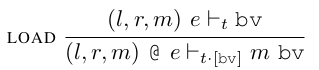
\includegraphics[scale = 0.7]{pictures/load.png}
\end{figure}

Ici, l'évaluation de l'expression \texttt{e} sur une configuration $(l,r,m)$ produit une fuite de la valeur $bv$. En haut nous retrouvons la notation de l'opération effectuée et au-dessous la formalisation de la fuite : $t \cdot [bv]$ signifie que la valeur $bv$ s'ajoute à la liste des fuites. Ce second exemple \ref{fig:instr_branchement} présente une opération de branchement en fonction de $e$ vers les instructions $l_1$ et $l_2$. On voit que la valeur est différente de zéro, ce qui nous produit une fuite vers l'instruction $l_1$. Cette fuite est à ajouter à notre liste $t$.

\begin{figure}[!ht]
  \caption{Instruction \texttt{branchement}}
  \label{fig:instr_branchement}
  \centering
  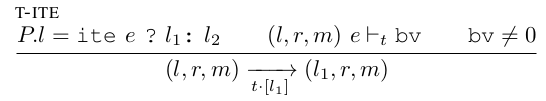
\includegraphics[scale = 0.7]{pictures/branchement.png}
\end{figure}

Nous pouvons retrouver l'ensemble des règles formelles en Annexe \ref{fig:ensemble_instr_formelles}.

\section{Analyse d'un programme}

Nous avons conçu un modèle pour contrôler ou détecter les erreurs. Nous pouvons maintenant concevoir notre analyse pour vérifier ce modèle sur un programme. Plusieurs techniques de vérification existent et nous allons les passer en revue : \cite{GeimerEvaluationsSideChannel}.\medbreak


\subsection*{Analyse statique}

Cette méthode consiste à déduire le fonctionnement d'un programme. Nous souhaitons vérifier que son fonctionnement respecte les propriétés de sécurité que nous avons définies. Cette analyse sans exécution réalise une simulation du programme en explorant les chemins d'exécution possibles. De fait, les résultats obtenus sont souvent approximés car une exploration totale peut se révéler irréalisable. Historiquement il s'agit de la première méthode étudiée et employée, en revanche elle a été dérivée en plusieurs approches.\medbreak

\paragraph{Non interférence.} Pour renforcer les résultats obtenus et réduire le nombre de faux positifs nous pouvons vérifier la propriété de non-interférence. Cette propriété est inhérente aux programmes. Un programme a des entrées et des sorties. Celles-ci peuvent être classées \textit{faibles} (peu importantes) ou \textit{hautes} (données secrètes, sensibles). Un programme est noninterférent si et seulement si pour n'importe quelle entrée faible le programme ressort la même sortie faible peu importe les entrées hautes qui peuvent être précisées.

Appliqué à une analyse statique pour la vérification de programme, la mesure des ressources employées par l'ordinateur permet d'avoir une sortie faible pour comparer le comportement d'un programme en fonction de ses entrées (ici considérées secrètes).

\paragraph{\textit{Self-Composition}}\footnote{Construction personnelle, le terme anglais est conservé.} La self-composition consiste à entrelacer deux exécutions d'un programme $P$ avec différents ensembles de variables secrètes dans un seul programme auto-composé $P;P'$. Des solveurs peuvent alors être utilisés pour vérifier la propriété de non-interférence. Cette approche a été utilisée par \citeauthor{ABPV13} \cite{ABPV13} pour vérifier manuellement des exemples limités, nécessitant de nombreuses annotations pour limiter l'explosion (quadratique) des états à comparer et explorer. \cite{binsecRel2019} emploie cette approche associée à des solveurs SMT pour vérifier uniquement les propriétés définies dans leur modèle. La restriction aux propriétés temps constant permet l'exploitation de cette méthode.

\paragraph{Systèmes de types} Cette approche diffère des précédentes car elle nécessite un travail supplémentaire du développeur. Il doit ajouter la spécification \texttt{secret} au valeurs employées pour que cette information se diffuse dans le compilateur et que des mesures adaptées soient effectuées au niveau du binaire. Cette approche est intéressante car elle permet une flexibilité plus importante lors de la production du code et permet de s'abstenir des contre-mesures décrites au chapitre \ref{chap:constantTimeSolution}; en revanche elle nécessite un compilateur spécialisé et aucune vérification sur le binaire produit n'est effectuée. 

\paragraph{Interprétation abstraite} Un programme est (généralement) trop complexe pour être entièrement formellement vérifié, donc il y a une sur approximation des états atteignables par l'analyse. Ainsi, si l'analyse approximée est sécurisée alors le programme est sécurisé. Cette approche se retrouve dans CacheAudit \cite{CacheAudit} : modélisation par un graphe de flot de l'état des caches, de la mémoire et des successions d'évènement.

\paragraph{Exécution symbolique} L'exécution symbolique consiste à exécuter le programme avec des entrées symboliques. Les chemins explorés sont associés à une formule logique, et un solveur vérifie si un ensemble de valeurs concrètes satisfait les formules générées. Cette méthode est utilisée pour vérifier l'absence de dépendance aux secrets dans les comportements temporels ou mémoire du programme.

\subsection*{Analyse dynamique}

L'analyse dynamique emploie la preuve par l'exemple pour garantir la sécurité du programme cible. Nous exécutons le programme et nous collectons sa trace : informations issues des évènements (accès mémoire, sauts,\etc) rencontrés au fur et à mesure de l'exécution. Les approches diffèrent dans la collecte et la production de ces traces.

\paragraph{Trace unique} Explorer tous les comportements d'un programme est coûteux en temps, et pour les besoins du développement il peut être préférable d'étudier quelques cas particuliers entièrement. Cette approche simplifie le modèle de l'attaquant et réalise sa vérification plus rapidement. \texttt{ctgrind} \cite{ctgrind} réutilise l'analyse dynamique de Valgrind pour vérifier les propriétés temps constant. Pour ajouter de la précision, il est possible d'utiliser l'exécution symbolique pour rejouer la trace avec le secret comme valeur symbolique et vérifier la violation du temps constant (CacheD \cite{CacheD}).

\paragraph{Comparaison de traces} Les tests statistiques peuvent vérifier si différents secrets induisent des différences significatives dans les traces enregistrées. Des outils comme DATA \cite{DATA1} ou MicroWalk \cite{MicroWalk} utilisent diverses méthodes statistiques ou d'apprentissage pour détecter et localiser les fuites. D'autres outils comme dudect \cite{dudect} enregistrent simplement le nombre total de cycles d'horloge et comparent leur distribution selon les secrets.

Le fuzzing peut aussi être utilisé pour trouver des entrées maximisant la couverture et la fuite via canal auxiliaire, comme dans ct-fuzz \cite{ctfuzz}.\medbreak


\textit{Ces modèles et ces approches permettent la mise en place d'outils d'analyse performants et innovants. Nous allons maintenant observer plus en détail leur fonctionnement.}

